\subsection{Traces écrites}
La principale trace écrite consistera à compléter au fur et à mesure des séances le tableau représenté à la figure~\ref{te} qui sera reproduit sur une feuille au format A3.

\newcommand{\echelle}{.985}
\begin{figure}[h!tbp]
\centering
\noindent\fcolorbox{black}{white}{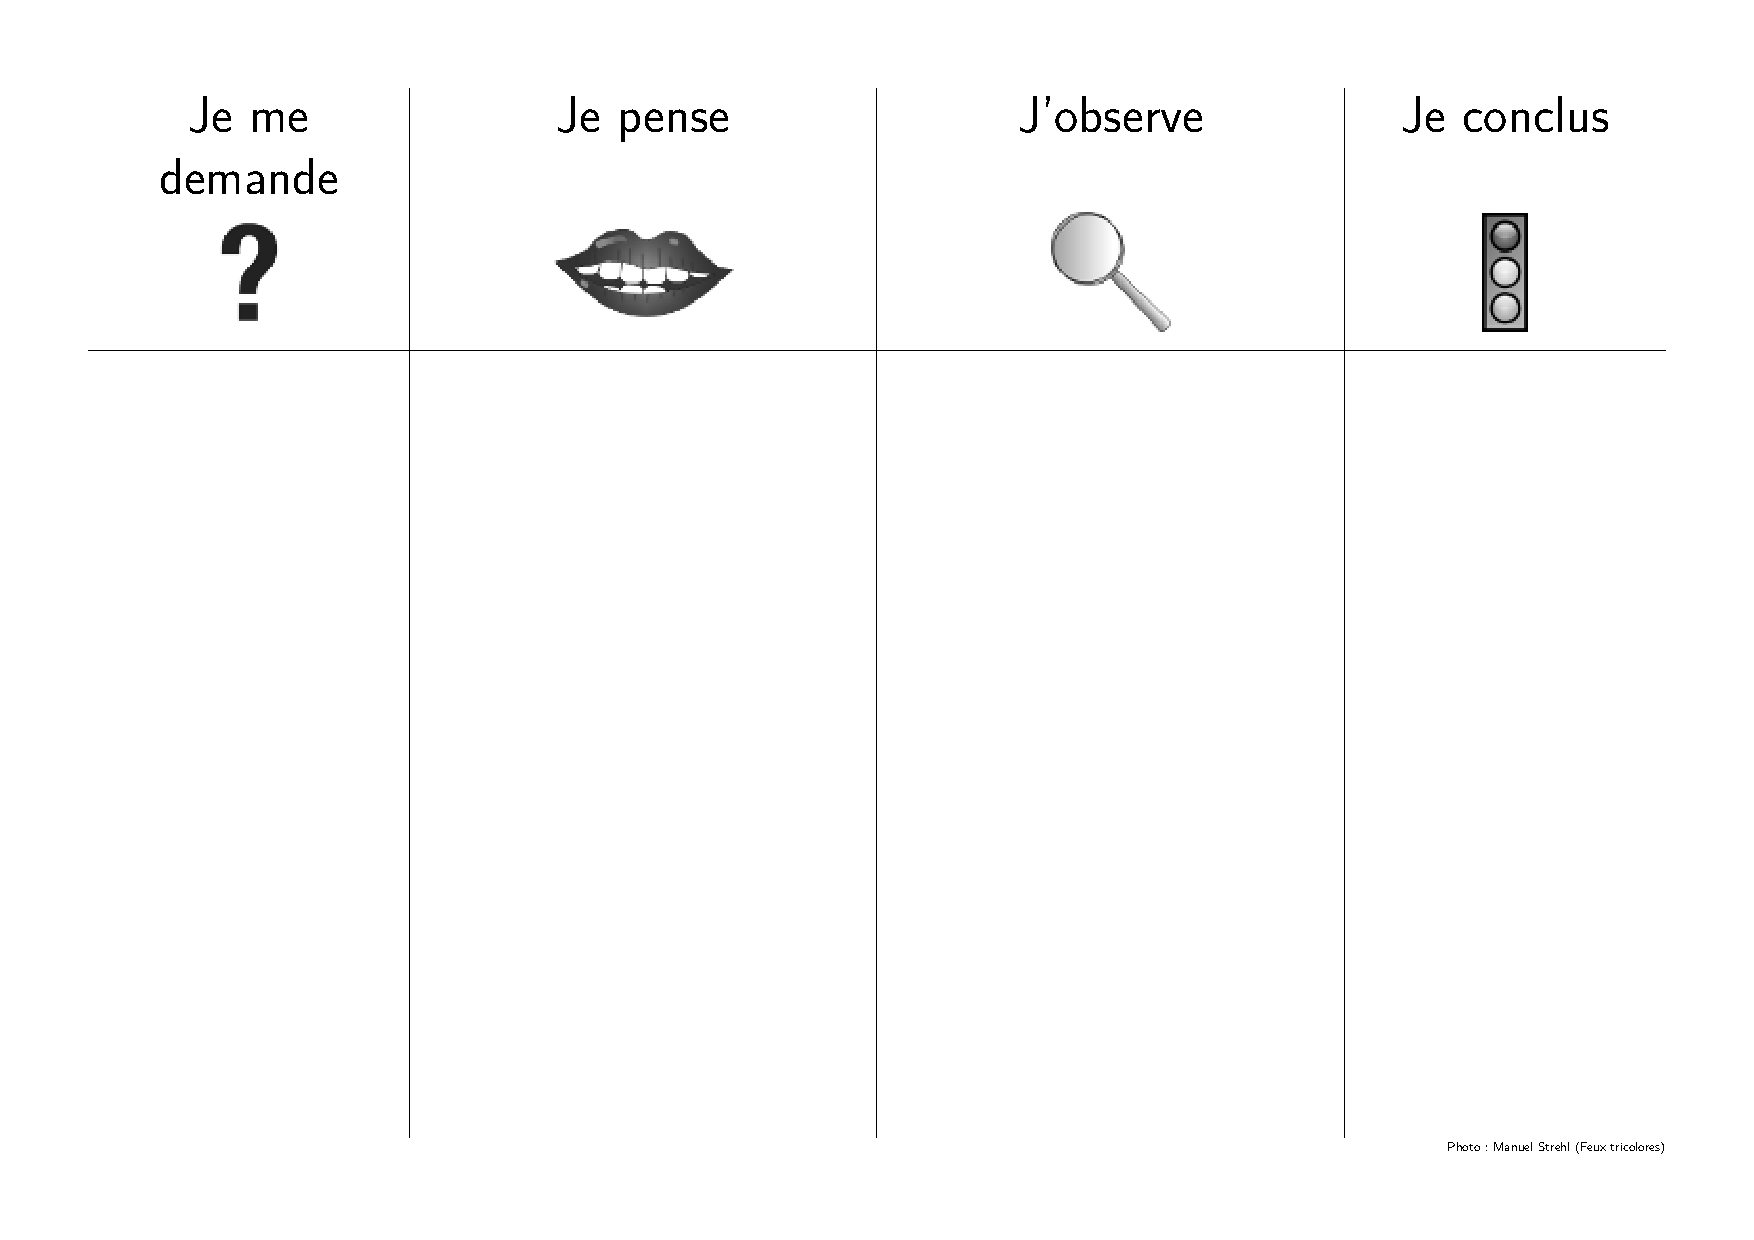
\includegraphics[width=\echelle\textwidth]{tex/TEaffiche.pdf}}
\caption{La démarche d’investigation en maternelle}
\label{te}
\end{figure}

Voici un aperçu des traces écrites.
\begin{description}
\item[Séance 1, \og \seancei \fg{}] Des photos du parc et de ce qu’on y trouve vont être prises par les enfants.
\item[Séance 2, \og \seanceii \fg{}] Des photos sont également prises une fois le tri réalisé. Elles iront enrichir le cahier de vie de la classe ou de l’enfant.
\item[Séance 3, \og \seanceiii \fg{}] Aucune trace écrite.
\item[Séance 4, \og \seanceiv \fg{}] Première et deuxième colonne du tableau : \textit{Je me demande} (Qu’est-ce qui pousse lorsque je l’enterre ?) et \textit{Je pense}.
\item[Séance 5, \og \seancev \fg{}] Pas de trace écrite. Néanmoins, chaque enfant aura un pot, avec l’étiquette de son prénom, ainsi qu’une vignette représentant ce qu’il a mis dans le pot.
\item[Séance 6, \og \seancevi \fg{}] Des photos ainsi que la troisième colonne du tableau : \emph{J’observe}.
\item[Séance 7, \og \seancevii \fg{}] Dernière colonne de tableau : \emph{Je conclus}.
\item[Séance 8, \og \seanceviii \fg{}] Dessin d’un gland germé dans le cahier de science.
\item[Séance 9, \og \seanceix \fg{}] Feuille d’évaluation.
\item[Séance 10, \og \seancex \fg{}] Pas de trace écrite.
\end{description}